%!TEX root = /Users/dedan/bccn/lab_rotations/johannes/report/report.tex
\chapter{Methods and Implementation} % (fold)

The basic idea was to use a computer vision system equipped with calibrated depth and RGB sensors. The additional availability of depth information makes the segmentation of the scene into potential objects much easier, since by providing distance information much of the ambiguity inherent to 2D image data can be resolved. The \emph{Kinect} camera system was chosen for the task because it is affordable, has depth and RGB sensors with up to 30Hz and the manufacturer provides a Software Development Kit which allows to access the camera through high-level programming languages.\\ \\
\begin{figure}[ht]
    \centering
        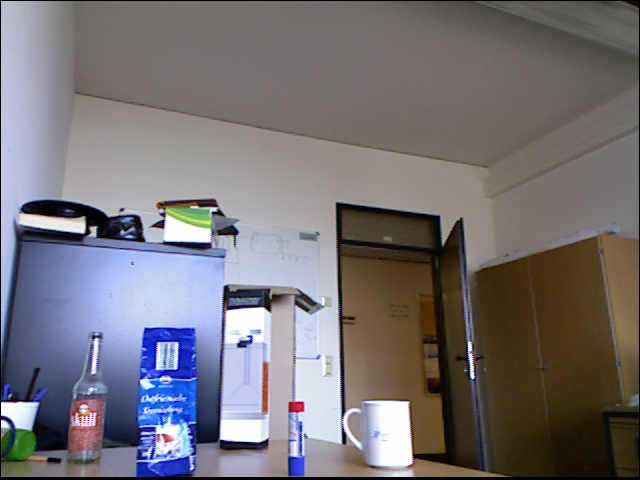
\includegraphics[width=5cm]{images/image.jpg}
        \hspace{0.1cm}
        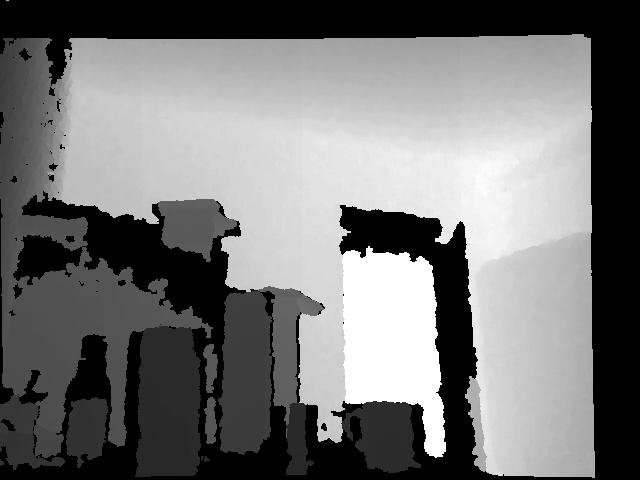
\includegraphics[width=5cm]{images/depth.jpg}
    \caption{The raw data coming from the Kinect camera. The left image shows the normal RGB image and the right one the depth information where distance is coded by the grayscale value.}
    \label{sg:fig:masked_patches}
\end{figure}

Some facts on the camera:
\begin{itemize}
    \item 8 bit RGB-Camera with resolution up to 1280x1024 @ 15 Hz or 640x480 @ 30 Hz
    \item 11 bit Depth-Camera with resolution of 640x480
    \item Depth sensor range: 0.8m - 6m (resolution decreases with distance)
\end{itemize} \\
After initial experiments with C++, Python was chosen because the high level logic of the software was much easier to be developed in this language and computationally expensive parts of the algorithm could still be executed in compiled programs as all of the used libraries provide python interfaces.
The code and its documentation is available by \cite{gabler:2011}\\ \\
The following libraries were used in the software:
\begin{description}
    \item[\textbf{OpenCV}] computer vision library
    \item[\textbf{numpy}] mathematics, numerics library for python
    \item[\textbf{libsiftfast}] scale Invariant Feature Transform
    \item[\textbf{FLANN}] approximate nearest neighbors calculation for object matching
\end{description}


\clearpage
\section{Histogram Clustering} % (fold)
\label{sg:sec:histogram_clustering}

The basic idea is to look for \emph{interesting layers} in the depth image. With the assumption that objects have only a narrow extension in depth it makes sense to look for accumulations of pixels that have similar depth values. In the histogram of the depth image, these accumulations are visible as \emph{hills} and serve as as a first guess for potential objects. The clustering approach is inspired by \cite{Jivet:tx} who also used histogram segmentation on depth images and is described in more detail in \ref{lst:clustering}. First a 600 bins histogram of the depth image is computed and then convoluted with a rectangular kernel in order to make it more smooth and to avoid small areas with equal distance. A kernel width of 5 points was chosen for the first half of the histogram and the second half of the histogram was smoothed with a wider kernel of 15 points to account for the decreasing resolution of the depth image (compare left and right image in \ref{sg:fig:images_cluster_bli_erode}). Subsequently the algorithm iterates over the histogram and separates the different \emph{hills} (clusters) which correspond to equally distant area. Which \emph{hill} is high enough to qualify as an interesting cluster can be tuned by the parameter \emph{perc} which gives the value for how much percent a value has to be lower then the last tip of a hill to choose this point as the right end of a cluster. A value of 20~\% gave good results with respect to our test environment. The following image (\ref{sg:fig:images_cluster_bli_erode}) shows the detected clusters in the histogram and also the corresponding pixel values which are coded by the same color.

\begin{figure}[ht]
    \centering
        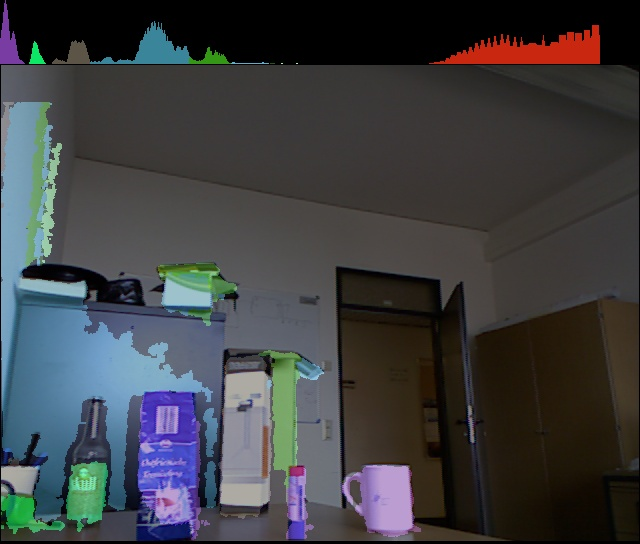
\includegraphics[width=0.45\textwidth]{images/cluster_bli_erode.jpg}
        \hspace{0.1cm}                      
        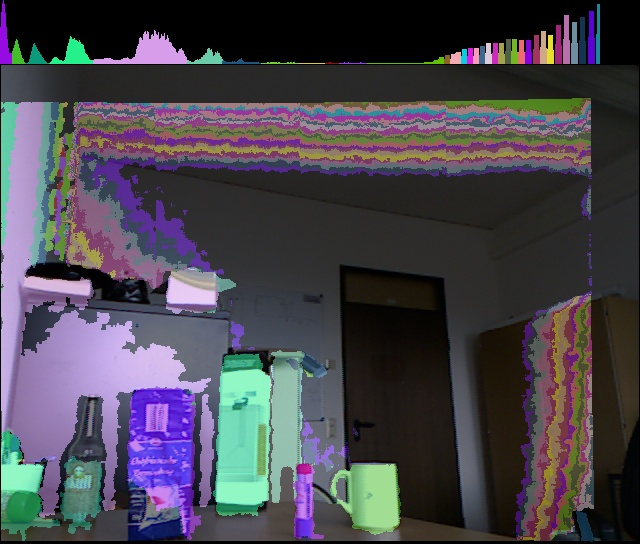
\includegraphics[width=0.45\textwidth]{images/histo_equal_smooth.jpg}        
    \caption{Left image: The top part of the figure shows the histogram of the depth image with its separation in different clusters (color coded). Areas with depth values falling in this cluster are then coded by the same color. In this plot the wider kernel is applied on the second half of the histogram.\\
    Right image: It shows the histogram clustering when the same kernel of 5 points width is used for the whole histogram. The resolution of the depth image decreases with distance and this leads to this many small valleys in the histogram. The valleys are missing values in the coarse resolution. To avoid that the clustering detects each of the valleys as a potential proto-object, a wider kernel of 15 points is used for smoothing of the second half of the histogram.}
    \label{sg:fig:images_cluster_bli_erode}
\end{figure}
\todo{beschreibung vertauschen oder bessere beschreibung}

\clearpage
\begin{listing}
    \lstset{ language=Pascal, numbers=left, numberstyle=\footnotesize, 
        stepnumber=5, numbersep=5pt}
    
    \begin{lstlisting}[frame=single]
compute histogram
prev_val = 0;
for each histogram value
begin
    if value > prev_value
    begin
        prev_value = value
    end
    
    if value < perc * prev_value
    begin
        extract the layer
        {all pixels with values in the between start_value and value}
        extract contours in the layer
    end
end
    \end{lstlisting}
    \caption{histogram clustering in pseudocode}
    \label{lst:clustering}
\end{listing}

% section histogram_clustering (end)




\clearpage
\section{Object detection and tracking} % (fold)
\label{sg:sec:dect_track}

The histogram clustering gives layers in which many pixels have similar depth values. Only the depth value is used for this first classification and in a second step spatial information is used to separate different objects located in one of the layers. This is done with the OpenCV function \emph{findContours} which implements the algorithm of \cite{Suzuki:1985tp}. An example of the result can be seen in Figure \ref{sg:fig:images_extracted_contours}.
\begin{figure}[ht]
    \centering
        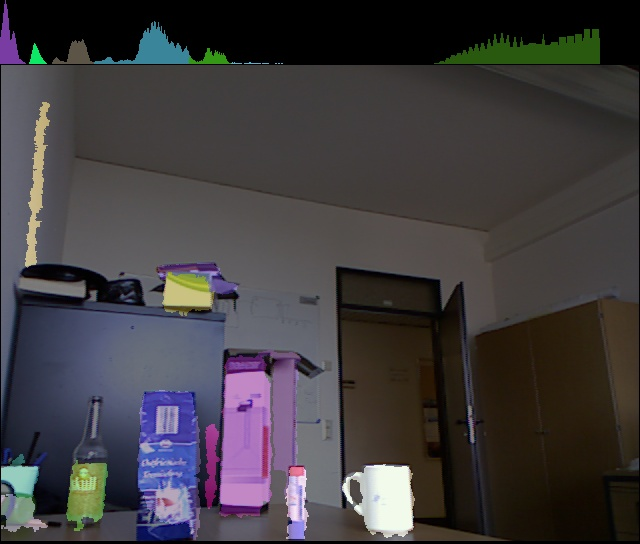
\includegraphics[width=0.6\textwidth]{images/extracted_contours.jpg}
    \caption{Each of the layers which are detected by the histogram clustering are scanned for spatially connected components. Each extracted contour is coded by a color. Note that contours which were previously detected only to be located in one layer of the depth image (Figure \ref{sg:fig:images_cluster_bli_erode}) are now recognized as separate objects.}
    \label{sg:fig:images_extracted_contours}
\end{figure}
Not all of these detected contours are potential objects. In the current implementation very simple criteria, such as minimal area, maximal area and contour complexity, are used to filter out irrelevant contours. In a more sophisticated implementation more complex filters could be applied, for example color homogeneity within a contour or prior knowledge about shapes that are likely (or unlikely) to appear in a certain scene.
The remaining contours are then kept in a list and are tracked over time. Again a very simple approach was applied to fulfill the goal of keeping the whole system realtime. For each frame the list of contours is computed as previously described. For each of the contours its minimum bounding rectangle is calculated and the overlap with the minimum bounding rectangle of all objects which are currently tracked is computed. If this overlap is larger than 50 \% of the size of the minimum bounding rectangle of the contour associated with the tracked object, the contour of the current frame will be the new contour of the tracked object. If a contour was not found to belong to any already known object it will be added to the tracking list as a new object. For a pseudocode description of the algorithm see listing \ref{lst:tracking}.
\clearpage
\begin{listing}
    \lstset{ language=Pascal, numbers=left, numberstyle=\footnotesize, 
        stepnumber=5, numbersep=5pt}
    
    \begin{lstlisting}[frame=single]
for each contour
begin
    compute minimum bounding rectangle
    for each already tracked object
    begin
        also compute minimum bounding rectangle
        compute rectangle overlap
        if overlap > 50 percent
        begin
            {object found within current frame}
            update contour of the object
        end
    end
    if contour not found in current list
    begin
        add it to tracking list as new object
    end
end
    \end{lstlisting}
    \caption{object tracking algorithm in pseudocode}
    \label{lst:tracking}
\end{listing}


% section dect_track (end)

\clearpage
\section{SIFT feature computation} % (fold)
\label{sg:sec:sift}

If a tracked object was stable found over more then N frames (N = 20 in the current implementation) it will be added to a scheduler list. This list is processed by a certain number of threads which compute SIFT-features (keypoints) on an object whenever the computational resources are available. Before the SIFT features are computed the extracted patch of the object (also the minimum bounding rectangle) is converted to a grayscale image. Furthermore the contour is used to mask the object. This avoids that the background of the images is wrongly attributed to an object. Image \ref{sg:fig:masked_patches} shows examples of these masked grayscale patches.
\begin{figure}[ht]
    \centering
        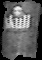
\includegraphics[width=2cm]{images/image_sift_12.jpg}
        \hspace{0.1cm}              
        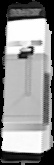
\includegraphics[width=2cm]{images/image_sift_42.jpg}
        \hspace{0.1cm}              
        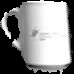
\includegraphics[width=2cm]{images/image_sift_69.jpg}
        \hspace{0.1cm}              
        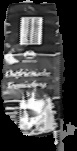
\includegraphics[width=2cm]{images/image_sift_87.jpg}
        \hspace{0.1cm}              
        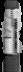
\includegraphics[width=2cm]{images/image_sift_89.jpg}
    \caption{Masked grayscale patches}
    \label{sg:fig:masked_patches}
\end{figure}

\begin{figure}[ht]
    \centering
        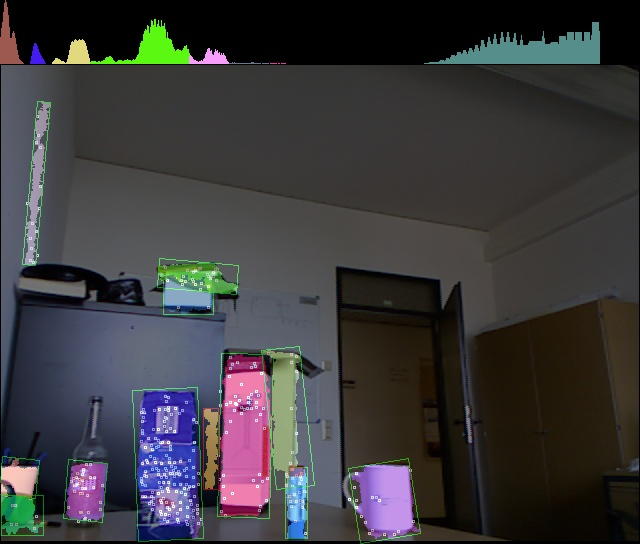
\includegraphics[width=0.7\textwidth]{images/contours_keypoints.jpg}
    \caption{SIFT features computed on the masked grayscale patches. Note that the masking avoids that features which belong to the background are assigned to the object.}
    \label{sg:fig:images_contours_keypoints}
\end{figure}

The computed SIFT-features per object are then matched again the database of previously recorded SIFT-features using the FLANN library. A keypoint is regarded as valid when the second best match in the database has more then 1.5 times the distance than the best match.
The available depth information can furthermore be used to check the validity of matched keypoints to exclude more false positive matches. Unfortunately the time-frame for this work did not allow to finish the implementation of this feature, but the idea would be to analyze the product the depth value at the keypoint location with the scale value of a keypoint. Having this two values it should be possible to asses how plausible it is to see a keypoint with a certain scale in a certain distance and this could help to sort out false-positive matchings.


% section sift (end)

% section methods (end)
